\exercisesheader{}

% 1 - acs

\eoce{\qt{ACS, Part I\label{acs}} Each year, the US Census Bureau surveys about 3.5 million households with The American Community Survey (ACS). Data collected from the ACS have been crucial in government and policy decisions, helping to determine the allocation of federal and state funds each year. Some of the questions asked on the survey are about their income, age (in years), and gender. The table below contains this information for a random sample of 20 respondents to the 2012 ACS. \footfullcite{data:acs:2012} \label{acs_age_income}
\begin{center}
\begin{minipage}[c]{0.4\textwidth}
{\small
\begin{tabular}{rrrl}
  \hline
 & Income & Age & Gender \\ 
  \hline
1 & 53,000 &  28 & male \\ 
  2 & 1600 &  18 & female \\ 
  3 & 70,000 &  54 & male \\ 
  4 & 12,800 &  22 & male \\ 
  5 & 1,200 &  18 & female \\ 
  6 & 30,000 &  34 & male \\ 
  7 & 4,500 &  21 & male \\ 
  8 & 20,000 &  28 & female \\ 
  9 & 25,000 &  29 & female \\ 
  10 & 42,000 &  33 & male \\ 
   \hline
\end{tabular}
}
\end{minipage}
\begin{minipage}[c]{0.4\textwidth}
{\small
\begin{tabular}{rrrl}
  \hline
 & Income & Age & Gender \\ 
  \hline
  11 & 670 &  34 & female \\ 
  12 & 29,000 &  55 & female \\ 
  13 & 44,000 &  33 & female \\ 
  14 & 48,000 &  41 & male \\ 
  15 & 30,000 &  47 & female \\ 
  16 & 60,000 &  30 & male \\ 
  17 & 108,000 &  61 & male \\ 
  18 & 5,800 &  50 & female \\ 
  19 & 50,000 &  24 & female \\ 
  20 & 11,000 &  19 & male \\ 
   \hline
\end{tabular}
}
\end{minipage}
\end{center}
\begin{parts}
\item Create a scatterplot of income vs. age, and describe the relationship between these two variables.
\item Now create two scatterplots: one for income vs. age for males and another for females.
\item How, if at all, do the relationships between income and age differ for males and females?
\end{parts}
}{}

% 2 - mlb

\eoce{\qt{MLB stats\label{mlb}} A baseball team's success in a season is usually measured by their number of wins. In order to win, the team has to have scored more points (runs) than their opponent in any given game. As such, number of runs is often a good proxy for the success of the team. The table below shows number of runs, home runs, and batting averages for a random sample of 10 teams in the 2014 Major League Baseball season. \footfullcite{data:MLB:2014}
\begin{center}
{\small
\begin{tabular}{rlrrr}
  \hline
 & Team & Runs & Home runs & Batting avg. \\ 
  \hline
1 & Baltimore &  705 &  211 & 0.256 \\ 
  2 & Boston &  634 &  123 & 0.244 \\ 
  3 & Cincinnati &  595 &  131 & 0.238 \\ 
  4 & Cleveland &  669 &  142 & 0.253 \\ 
  5 & Detroit &  757 &  155 & 0.277 \\ 
  6 & Houston &  629 &  163 & 0.242 \\ 
  7 & Minnesota &  715 &  128 & 0.254 \\ 
  8 & NY Yankees &  633 &  147 & 0.245 \\ 
  9 & Pittsburgh &  682 &  156 & 0.259 \\ 
  10 & San Francisco &  665 &  132 & 0.255 \\ 
   \hline
\end{tabular}
}
\end{center}
\begin{parts}
\item Draw a scatterplot of runs vs. home runs.
\item Draw a scatterplot of runs vs. batting averages.
\item Are home runs or batting averages more strongly associated with number of runs? Explain your reasoning.
\end{parts}
}{}

% 3 - fiber_cereal

\eoce{\qt{Fiber in your cereal \label{fiber_cereal}} The Cereal FACTS report provides information on nutrition content of cereals as well as who they are targeted for (adults, children, families). We have selected a random sample of 20 cereals from the data provided in this report. Shown below are the fiber contents (percentage of fiber per gram of cereal) for these cereals. \footfullcite{Harris:2012}
\begin{center}
\begin{minipage}[c]{0.49\textwidth}
{\small
\begin{tabular}{rlr}
  \hline
 & Brand & Fiber \% \\ 
  \hline
1 & Pebbles Fruity & 0.0\% \\ 
  2 & Rice Krispies Treats & 0.0\% \\ 
  3 & Pebbles Cocoa & 0.0\% \\ 
  4 & Pebbles Marshmallow & 0.0\% \\ 
  5 & Frosted Rice Krispies & 0.0\% \\ 
  6 & Rice Krispies  & 3.0\% \\ 
  7 & Trix  & 3.1\% \\ 
  8 & Honey Comb  & 3.1\% \\ 
  9 & Rice Krispies Gluten Free & 3.3\% \\ 
  10 & Frosted Flakes  & 3.3\% \\ 
   \hline
\end{tabular}
}
\end{minipage}  
 \begin{minipage}[c]{0.49\textwidth}
{\small
\begin{tabular}{rlr}
  \hline
 & Brand & Fiber \% \\ 
   \hline 
  11 & Cinnamon Toast Crunch & 3.3\% \\ 
  12 & Reese's Puffs  & 3.4\% \\ 
  13 & Cheerios Honey Nut & 7.1\% \\ 
  14 & Lucky Charms  & 7.4\% \\ 
  15 & Pebbles Boulders Chocolate PB & 7.4\% \\ 
  16 & Corn Pops  & 9.4\% \\ 
  17 & Frosted Flakes Reduced Sugar & 10.0\% \\ 
  18 & Clifford Crunch  & 10.0\% \\ 
  19 & Apple Jacks  & 10.7\% \\ 
  20 & Dora the Explorer  & 11.1\% \\ 
   \hline
\end{tabular}
}
\end{minipage}  
\end{center}
\begin{parts}
\item Create a stem and leaf plot of the distribution of the fiber content of these cereals.
\item Create a dot plot of the fiber content of these cereals.
\item Create a histogram and a relative frequency histogram of the fiber content of these cereals.
\item What percent of cereals contain more than 7\% fiber?
\end{parts}
}{}

% 4 - sugar_cereal

\eoce{\qt{Sugar in your cereal\label{sugar_cereal}} The Cereal FACTS report from Exercise~\ref{fiber_cereal} also provides information on sugar content of cereals. We have selected a random sample of 20 cereals from the data provided in this report. Shown below are the sugar contents (percentage of sugar per gram of cereal) for these cereals.
\begin{center}
\begin{minipage}[c]{0.49\textwidth}
{\small
\begin{tabular}{rlr}
  \hline
 & Brand & Sugar \% \\ 
  \hline
1 & Rice Krispies Gluten Free & 3\% \\ 
  2 & Rice Krispies  & 12\% \\ 
  3 & Dora the Explorer  & 22\% \\ 
  4 & Frosted Flakes Red. Sugar & 27\% \\ 
  5 & Clifford Crunch  & 27\% \\ 
  6 & Rice Krispies Treats & 30\% \\ 
  7 & Pebbles Boulders Choc. PB & 30\% \\ 
  8 & Cinnamon Toast Crunch & 30\% \\ 
  9 & Trix  & 31\% \\ 
  10 & Honey Comb  & 31\% \\ 
   \hline
\end{tabular}
}
\end{minipage}  
 \begin{minipage}[c]{0.49\textwidth}
{\small
\begin{tabular}{rlr}
  \hline
 & Brand & Sugar \% \\ 
   \hline 
  11 & Corn Pops  & 31\% \\ 
  12 & Cheerios Honey Nut & 32\% \\ 
  13 & Reese's Puffs  & 34\% \\ 
  14 & Pebbles Fruity & 37\% \\ 
  15 & Pebbles Cocoa & 37\% \\ 
  16 & Lucky Charms  & 37\% \\ 
  17 & Frosted Flakes  & 37\% \\ 
  18 & Pebbles Marshmallow & 37\% \\ 
  19 & Frosted Rice Krispies & 40\% \\ 
  20 & Apple Jacks  & 43\% \\
   \hline
\end{tabular}
}
\end{minipage}  
\end{center}
\begin{parts}
\item Create a stem and leaf plot of the distribution of the sugar content of these cereals.
\item Create a dot plot of the sugar content of these cereals.
\item Create a histogram and a relative frequency histogram of the sugar content of these cereals.
\item What percent of cereals contain more than 30\% sugar?
\end{parts}
}{}

% 5 - mammal_life_spans

\eoce{\qt{Mammal life spans\label{mammal_life_spans}} Data were collected on life spans (in 
years) and gestation lengths (in days) for 62 mammals. A scatterplot of life span versus 
length of gestation is shown below. \footfullcite{Allison+Cicchetti:1975}

\noindent\begin{minipage}[c]{0.44\textwidth}
\begin{parts}
\item What type of an association is apparent between life span and length of gestation?
\item What type of an association would you expect to see if the axes of the plot were reversed, i.e. if we plotted length of gestation versus life span?
\item Are life span and length of gestation independent? Explain your reasoning.
\end{parts}
\end{minipage}
\begin{minipage}[c]{0.55\textwidth}
\begin{center}
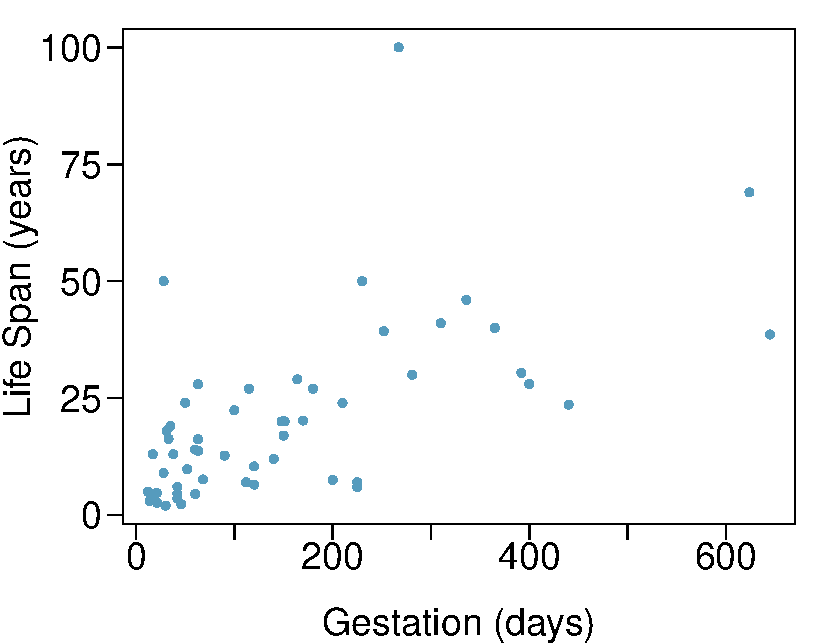
\includegraphics[width = 0.86\textwidth]{ch_summarizing_data/figures/eoce/mammal_life_spans/mammal_life_spans_scatterplot.pdf}
\end{center}
\end{minipage}
}{}

% 6 - association_plots

\eoce{\qt{Associations\label{association_plots}}
Indicate which of the plots show
(a)~a positive association,
(b)~a negative association, or
(c)~no~association.
Also determine if the positive and negative associations
are linear or nonlinear.
Each part may refer to more than one plot.
\begin{center}
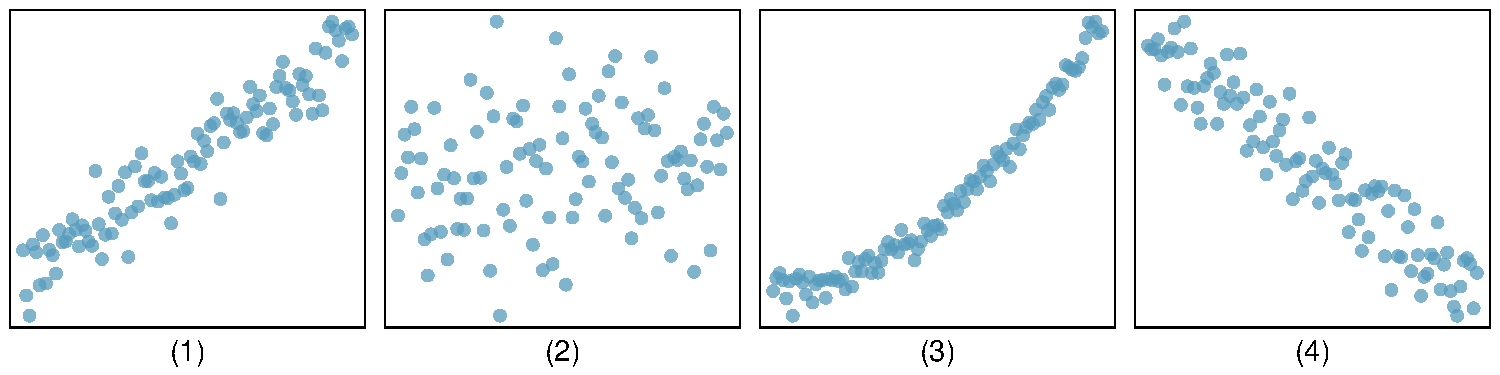
\includegraphics[width = 0.95\textwidth]{ch_summarizing_data/figures/eoce/association_plots/association_plots.pdf}
\end{center}
}{}
